The whole project encompasses different libraries, prototypes and applications.
This chapter describes the design of each part of the product in detail,
and documents the various approaches taken into consideration.

\section{System overview}

The system consists of:
\begin{description}
	\item[Libraries:] Social library, Communication library
	\item[Applications:] Jacket application, other applications
	\item[(U.I.) Prototypes:] Jacket prototype, other prototypes
\end{description}

The figure \ref{fig:design-toplevel} illustrates the overall system architecture.

\begin{figure}[h!]
	\centering 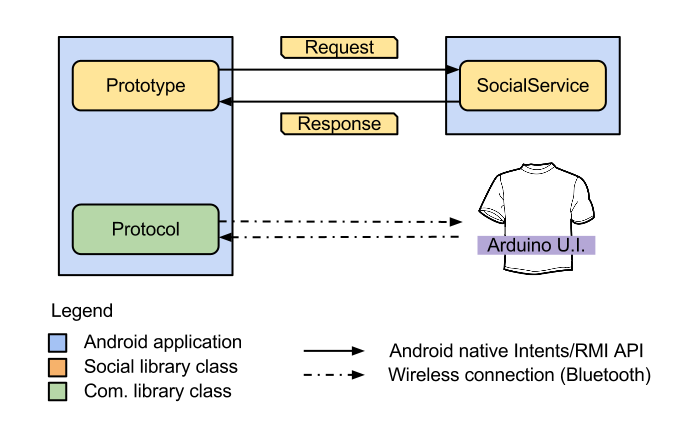
\includegraphics[scale=0.55]{img/design-toplevel.png}
	\caption{System architecture overview}
	\label{fig:design-toplevel}
\end{figure}


\section{System design}
\label{sec:system-design}
As the requirements for the product were not set early on by the customer, a lot of effort
was put into producing working prototypes to show during the meetings in order to receive
as much feedback as possible and identify the ideas the customer had in mind. This would provide information on
what was needed to proceed with system design. At some point, after roughly one month,
we understood that we were going in the wrong direction, and that our design wouldn't satisfy
the requirements the customer had mentioned. The design of some parts of the system had to be revised.

\subsection{First design}
Our first system design was based on the scenario where the user would download the Jacket
and the social applications, browse for some content from within the social application
and actively send it to the tangible user interface (the jacket) by pressing a 'share' button.
This scenario is illustrated in figure \ref{fig:design-usecase1}.

\begin{figure}[h!]
	\centering 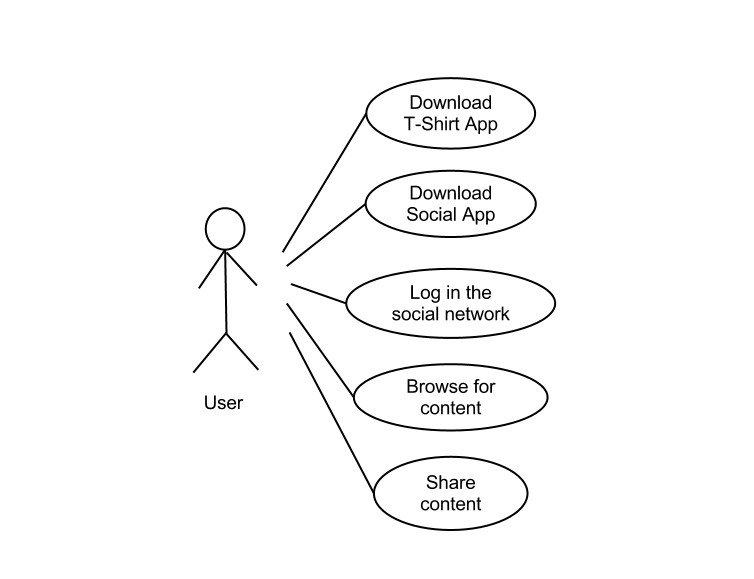
\includegraphics[scale=0.35]{img/design-usecase1}
	\caption{Use case for the product (first design)}
	\label{fig:design-usecase1}
\end{figure}

Please note that in this scenario the user is required to actively send data from
the social application (which acts as a Facebook client) to the jacket application,
which is merely capable of receiving. Also, both are implemented as Android applications.

The figure \ref{fig:design-resp} illustrates the communication between the applications.

\begin{figure}[h!]
	\centering 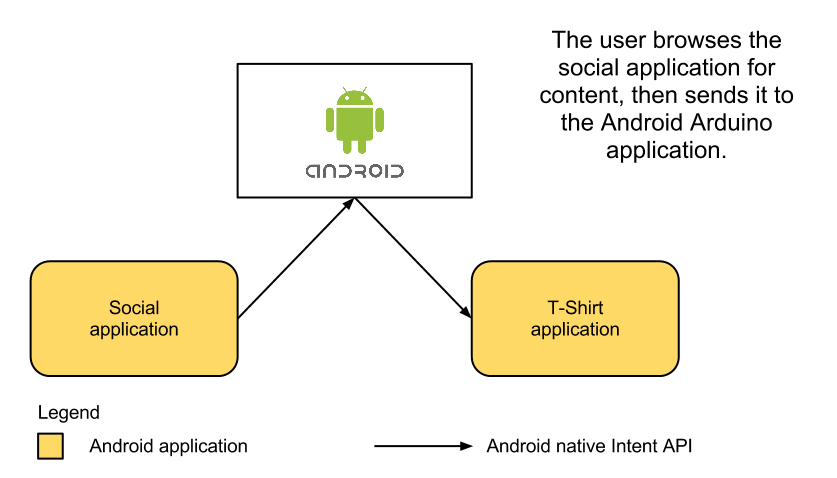
\includegraphics[scale=0.35]{img/design-resp.png}
	\caption{Communication diagram (first design)}
	\label{fig:design-resp}
\end{figure}


\subsection{Second design}
It turned out that the user was not supposed to browse for social content and actively send it 
to the jacket application. Instead, after downloading the software, he would just setup a set of rules
specifying the behavior of the Jacket. This scenario is illustrated in figure \ref{fig:design-usecase2}

\begin{figure}[h!]
	\centering 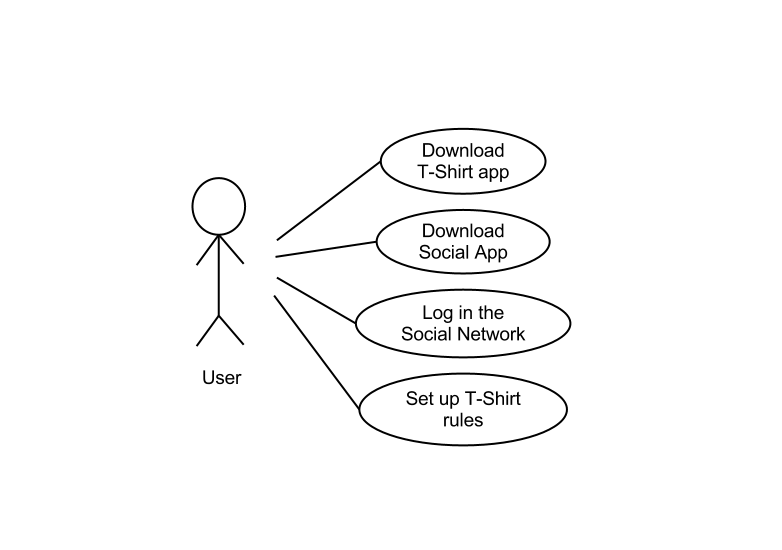
\includegraphics[scale=0.35]{img/design-usecase2}
	\caption{Use case for the product (second design)}
	\label{fig:design-usecase2}
\end{figure}

This new scenario made clear that the jacket and social applications had to be re-designed to support new requirements.

\begin{description}

	\item [Jacket application:] A user interface, implemented as an Android application,
	that the user would use to setup the rules for the jacket. The application also needed a
	background component (such as an Android service or Thread) that would 'ask' the required
	information to the social service.

	\item [Social application:] An Android service that would run in the background, without user interaction,
	to fetch data from the social networks and return it to the T-shirt application.
	The service should also have a user interface in order to let the user authenticate and
	enable/disable the service itself.

\end{description}

It also implied that a mechanism to request and exchange social content, as well as the necessary
data models abstractions, had to be provided by the Social library. The figure \ref{fig:design-reqresp}
illustrates the communication between the services and the appconfigurelications.

\begin{figure}[h!]
	\centering 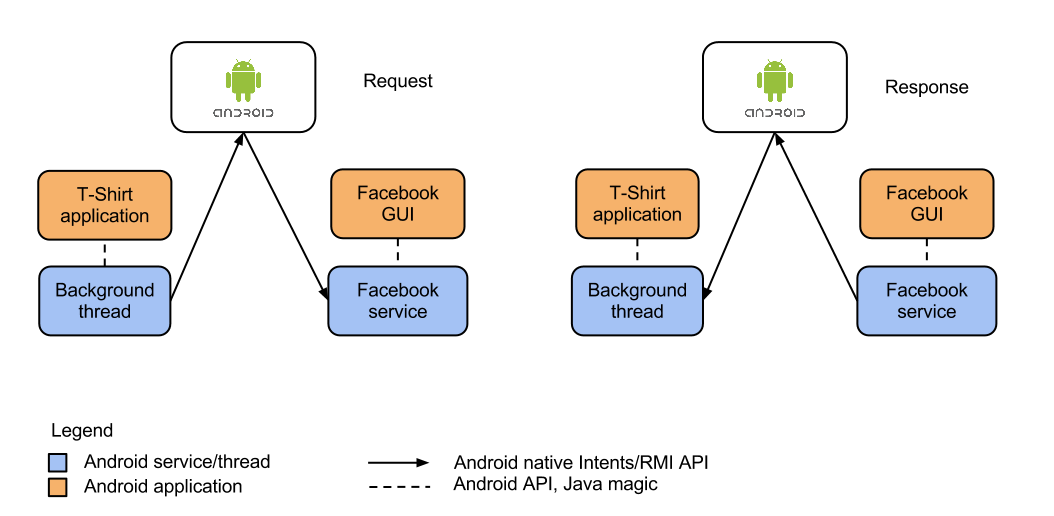
\includegraphics[scale=0.35]{img/design-reqresp.png}
	\caption{Communication diagram (second design)}
	\label{fig:design-reqresp}
\end{figure}

The Jacket application is now 'asking' the social application for a specific content.
This happens in the background, without user interaction.

\subsubsection{Sequence diagram}
This sequence diagram shown in figure \ref{fig:design-sequence} shows a sample communication between a social app and the jacket application.
The jacket application requests the list of friends of the logged in user from Facebook.

\begin{figure}[h!]
	\centering 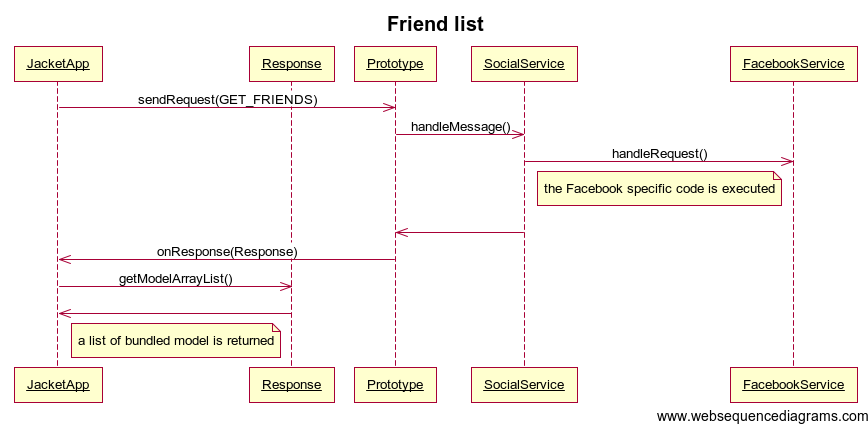
\includegraphics[width=1.0\textwidth]{img/design-sequence.png}
	\caption{Sequence diagram}
	\label{fig:design-sequence}
\end{figure}


\section{Libraries}

\subsection{The Social library}
The Social library is the link between the Android applications that control the
behavior of TUI prototypes and social networks. It provides abstractions for
many common concepts found in different social networks like Facebook, Twitter
and OpenSocial. This allows third-party developers to use these models seamlessly
between different social networks and extend them to possibly support others.
It also defines and implements a set of classes to allow Android applications
and services to exchange such data models. This mechanism is based on Android's
native inter-process communication API (both intents, and message-based \newline
communication). The figures \ref{fig:social-classes} and \ref{fig:model-classes}
illustrate the most relevant classes of the library.

\begin{figure}[h!]
	\centering 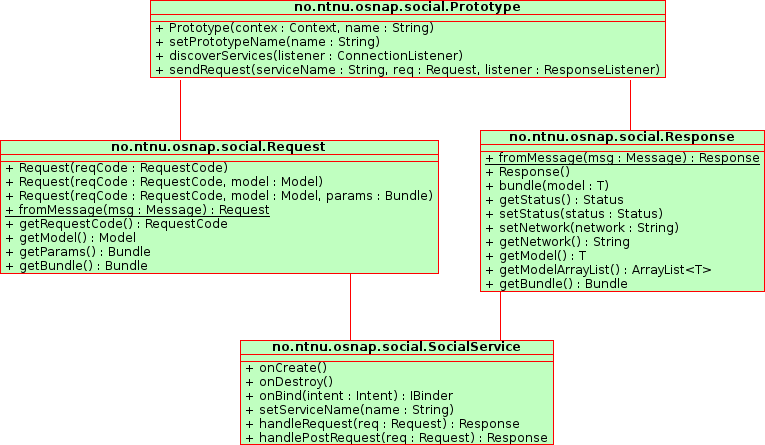
\includegraphics[scale=0.7]{img/architecture-socialclasses.png}
	\caption{Social library core classes}
	\label{fig:social-classes}
\end{figure}

\begin{figure}[h!]
	\centering 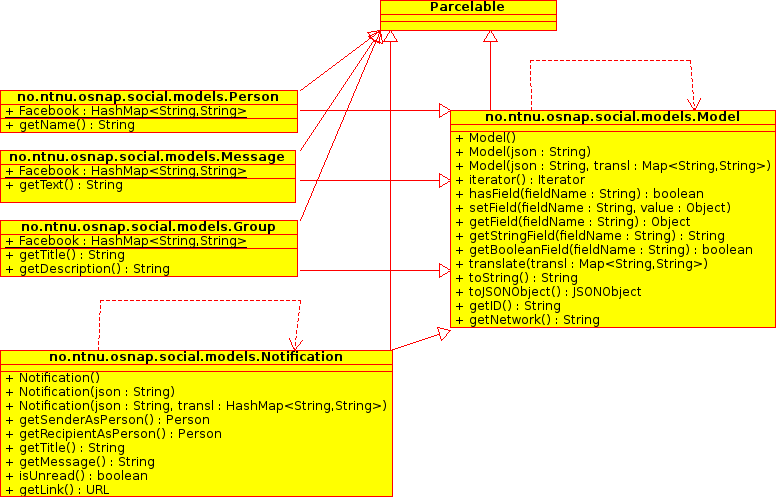
\includegraphics[scale=0.7]{img/architecture-modelclasses.png}
	\caption{Social library data models}
	\label{fig:model-classes}
\end{figure}


\subsection{The Communication library}
This library consists of a Java library (implemented on Android) and an Arduino firmware (figure \ref{fig:comlib-diagram}),
both implementing the ComLib protocol. The Java library provides a set of classes that simplify the connection to Arduino
devices that run the Communication library Arduino firmware. The library also implements a mechanism to request a list of 
services (components) the remote device supports and any software download links associated with the remote device. A service might
be a sensor, a lamp, display screen, etc, while download links are represented as an URL link. All this meta information is stored
on in the firmware on the remote device as raw text using the JSON format. This meta-data can also be stored and retrieved
in a QR code or other plain text formats.

\begin{figure}[h!]
	\centering 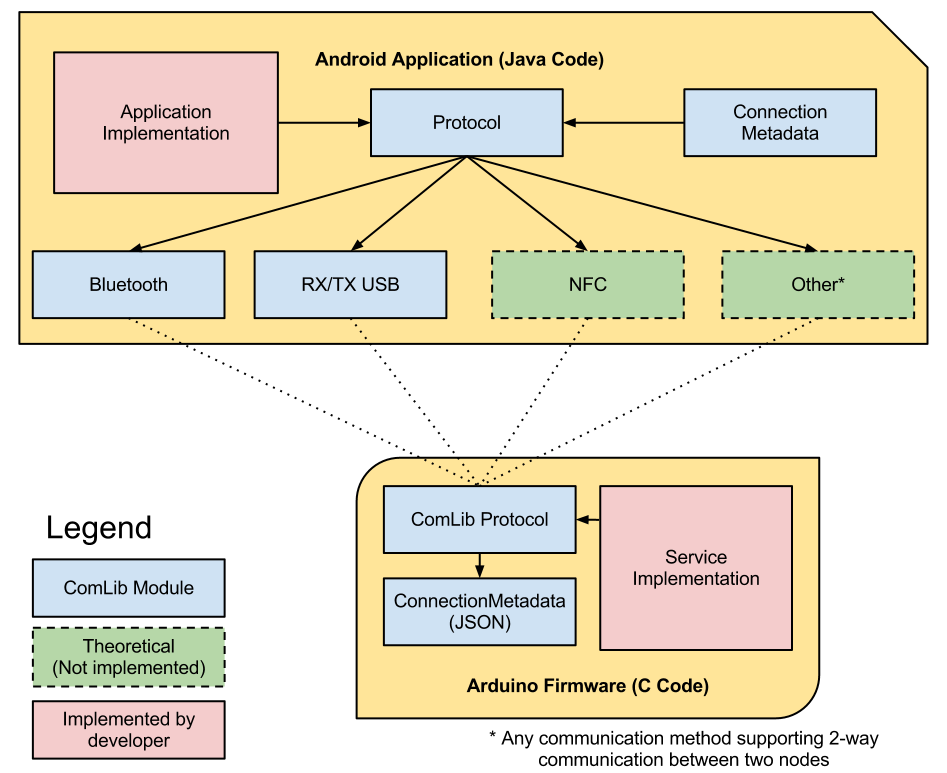
\includegraphics[scale=0.4]{img/comlib-diagram.png}
	\caption{Diagram for the Communication Library design}
	\label{fig:comlib-diagram}
\end{figure}

\subsubsection{The ComLib protocol}
The protocol is a basic set of rules that define how devices can communicate to the Arduino.
The ComLib protocol itself was designed by us, and has seen much changes in terms of which instructions were to be included,
and how the communication was to be executed. With the current design the Arduino cannot initiate the communication,
but is instead a passive device. For all instructions sent by any device to the Arduino, the Arduino sends a response,
either to acknowledge that it is finished executing the corresponding tasks, or the actually return the required
information in the "Content" field. An overview of the current instructions in the protocol can be seen in Table~\ref{tbl:opcodes}.

\begin{table}[h!]
	\begin{tabular}{ | c | c | p{1.5cm} | p{1.7cm} | p{6cm} |}
		\hline
		\textbf{Name} & \textbf{OPCODE} & \textbf{Flag} & \textbf{Content} & \textbf{Description} \\
		\hline
		Ping & 0x00 & N/A & N/A & Pings the arduino, to check that it's there \\
		\hline
		Text & 0x01 & N/A & Text to send & Sends text to the arduino, which then displays it depending on the implementation on the Arduino \\
		\hline
		Sensor & 0x02 & Sensor number & N/A & Requests sensor information from the arduino \\
		\hline
		Pin pulse & 0x03 & Pin number & N/A & Sends a 500ms pulse on the specified pin \\
		\hline
		Pin read & 0x04 & Pin number & N/A & Reads the current digital state of the specified pin on the arduino \\
		\hline
		Pin write & 0x05 & Pin number & Pin value (0 or 1) & Writes a digital state of a pin on the arduino \\
		\hline
		Response & 0xFE & Opcode & Response content & A response to a previous instruction, where the flag is the opcode for which it is the response to \\
		\hline
		Reset & 0xFF & N/A & N/A & Resets the arduino \\
		\hline
	\end{tabular}
	\caption{Overview of protocol's instructions}
	\label{tbl:opcodes}
\end{table}

\subsubsection{Arduino firmware implementation}
On the Arduino, all code related to our protocol is abstracted into a ComputerSerial library.
This library is a very basic state machine which processes single bytes received (see Figure~\ref{fig:arduino_states}).
The user of this library can register local methods to be called with RPC when the corresponding instruction is called.
The instructions follow strict rules on how they are constructed (see Table~\ref{tbl:instr_struct} for sizes of the different parts).
Each instruction has to start with a "start-byte" which is always 0xFF (255 decimal). The next part is the size, which tells the number of bytes to come for this instruction (including the size byte itself). The rest is defined from which instruction is sent, but it is important to
remember that the content cannot be empty, and has to at least contain one byte. This byte however, is not necessarily read or used.

The following figure \ref{fig:arduino_states} illustrates the Arduino state machine:

\begin{figure}[H]
	\centering
	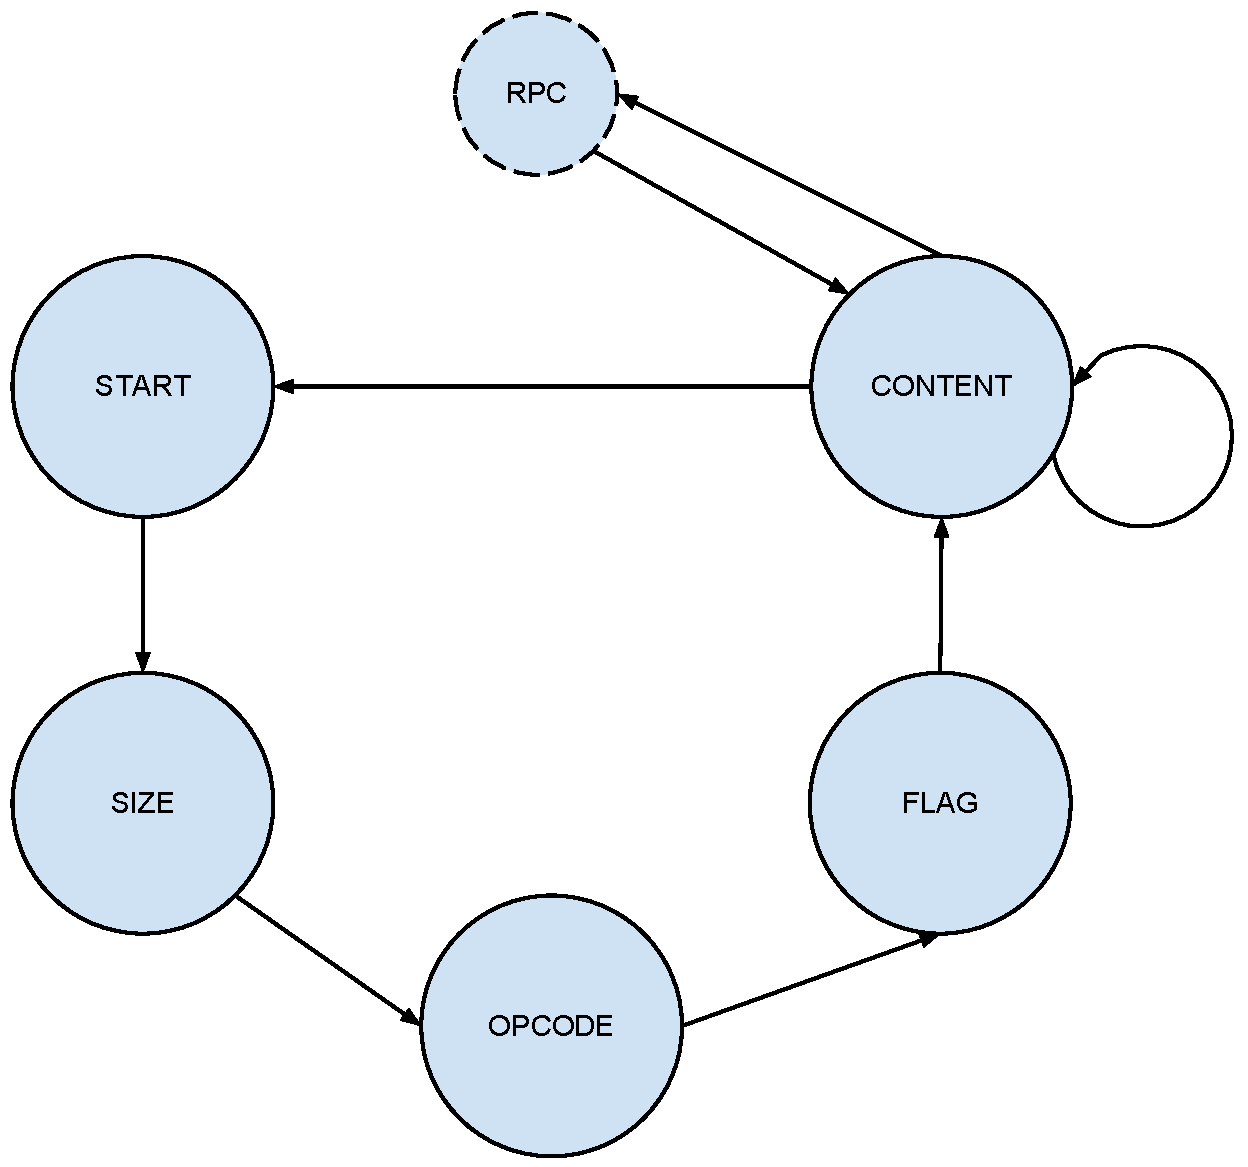
\includegraphics[scale=0.5]{img/arduino_state-machine.pdf}
	\caption{The Arduino state-machine}
	\label{fig:arduino_states}
\end{figure}

\begin{table}[H]
	\begin{tabular}{c|c|c|c|c|c|}
		\cline{2-6}
		& \textbf{Start-byte} & \textbf{Size} & \textbf{Opcode} & \textbf{Flag} & \textbf{Content} \\
		\hline
		\multicolumn{1}{|c|}{\textbf{Size}} & 1 & 1 & 1 & 1 & 1-252 \\
		\hline
	\end{tabular}
	\caption{Byte-structure of instructions}
	\label{tbl:instr_struct}
\end{table}


\section{Applications}
This section describes the various Android applications developed in detail.

\subsection{oSNAP Generic Application} \label{section:app-generic}
\begin{wrapfigure}{l}{20mm}
	\centering 
\includegraphics[scale=0.25]{img/app-generic}
\end{wrapfigure}
This application allows the user to scan a QR code and connect via Bluetooth to a remote TUI prototype.
It will then retrieve additional metadata from the remote device and use it to present a list of all the
functionality supported. The user can then test each feature with the click of a button,
and download the prototype specific application from a link to the oSNAP market.
The idea is that the user can use this application to scan various oSNAP products and retrieve
additional information or software for that specific product. This application was initially used to test
the TUI prototypes but was later converted to a 'real' application as the client request.
The application startup screen is showed in figure \ref{fig:osnap-generic}.

\begin{figure}[h!]
	\centering 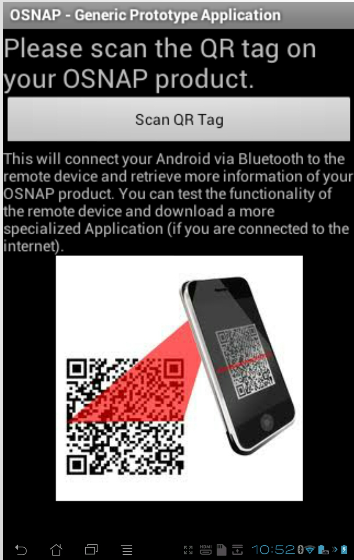
\includegraphics[scale=0.4]{img/osnap-generic}
	\caption{Screenshot of the Generic oSNAP Application}
	\label{fig:osnap-generic}
\end{figure}

\subsection{oSNAP Jacket Application} \label{section:app-jacket}
\begin{wrapfigure}{l}{20mm}
	\centering 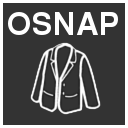
\includegraphics[scale=0.25]{img/app-jacket}
\end{wrapfigure}
This application controls the behavior of the Jacket prototype (\ref{fig:jacketapp-overview},
using both the Social and Comm. libraries. It allows the user to setup rules
which control the various devices embedded in the Jacket based on data retrieved
from social networks. One example could be a rule to play a sound effect through
the Jacket speaker whenever a notification from a certain user is received on
Facebook.

\begin{figure}[H]
	\centering 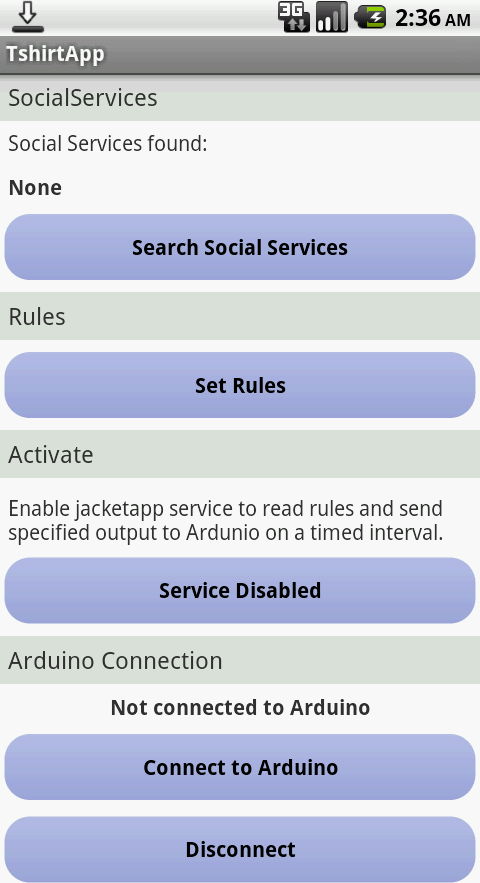
\includegraphics[scale=0.35]{img/jacketapp-overview}
	\caption{Screenshot of the main screen in the oSNAP Jacket Application}
	\label{fig:jacketapp-overview}
\end{figure}

As discussed in chapter \ref{sec:system-design} the T-shirt application design had to be reviewed after roughly one month.

\begin{figure}[H]
	\centering 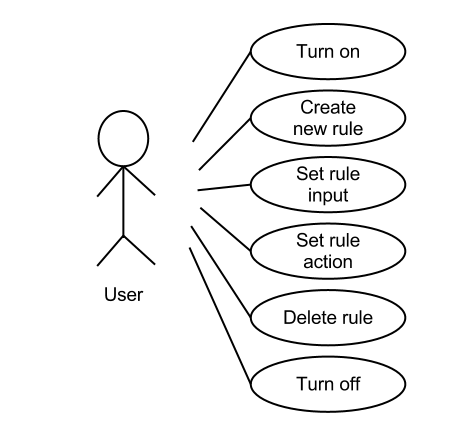
\includegraphics[scale=0.35]{img/design-tshirtappusecase2}
	\caption{Use case for the T-shirt application}
	\label{fig:design-tshirtappusecase2}
\end{figure}

For completeness we present the previous application use case in figure \ref{fig:design-tshirtappusecase1}

\begin{figure}[H]
	\centering 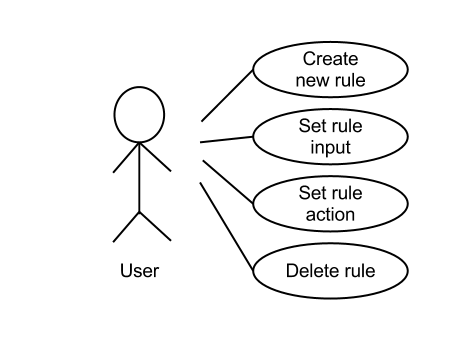
\includegraphics[scale=0.35]{img/design-tshirtappusecase1}
	\caption{Initial use case for the T-shirt application}
	\label{fig:design-tshirtappusecase1}
\end{figure}

\subsection{oSNAP Facebook application} \label{section:service-fb}
\begin{wrapfigure}{l}{20mm}
	\centering 
\includegraphics[scale=0.25]{img/app-fb}
\end{wrapfigure}
The Facebook application is an Android application that that replies
TUI prototype applications' requests by providing a Social library's 'Social service'
Facebook-specific implementation.

As discussed in chapter \ref{sec:system-design} the Facebook application design had to be reviewed after roughly one month.

\begin{figure}[H]
	\centering 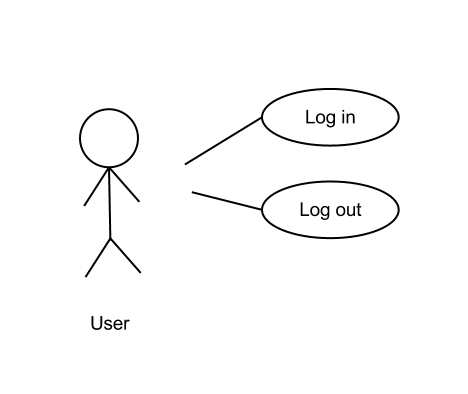
\includegraphics[scale=0.35]{img/design-socialappusecase2}
	\caption{Use case for the Social application}
	\label{fig:design-socialappusecase2}
\end{figure}

For completeness we present the previous application use case in figure \ref{fig:design-socialappusecase1}.

\begin{figure}[H]
	\centering 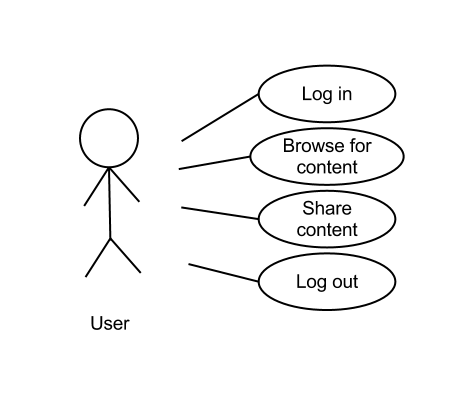
\includegraphics[scale=0.35]{img/design-socialappusecase1}
	\caption{Initial use case for the Social application}
	\label{fig:design-socialappusecase1}
\end{figure}

\subsection{oSNAP Temperature Application}
\begin{wrapfigure}{l}{20mm}
	\centering 
\includegraphics[scale=0.25]{img/app-temp}
\end{wrapfigure}
This application allows the user to connect to an Arduino thermometer device wirelessly through Bluetooth (read more about the 
temperature prototype in section \ref{section:prototype-temp}). This is done by scanning a QR code to retrieve the mac address
of the remote device. The application can then retrieve temperature updates to display them directly on the Android or automatically 
upload temperature updates to Facebook. This application demonstrates that the libraries work independently
and are not hard-coded for one application. It also shows that the ComLib supports two-way communication.
In the planning stage of this prototype, a paper prototype (see figure~\ref{fig:prototype2-paper}) was showed to the
customer. Due to some problems to get the initial design to work properly, the GUI was revised (see
figure~\ref{fig:prototype2-gui}) to make it more user friendly and visually appealing.

\begin{figure}[H]
\centering 
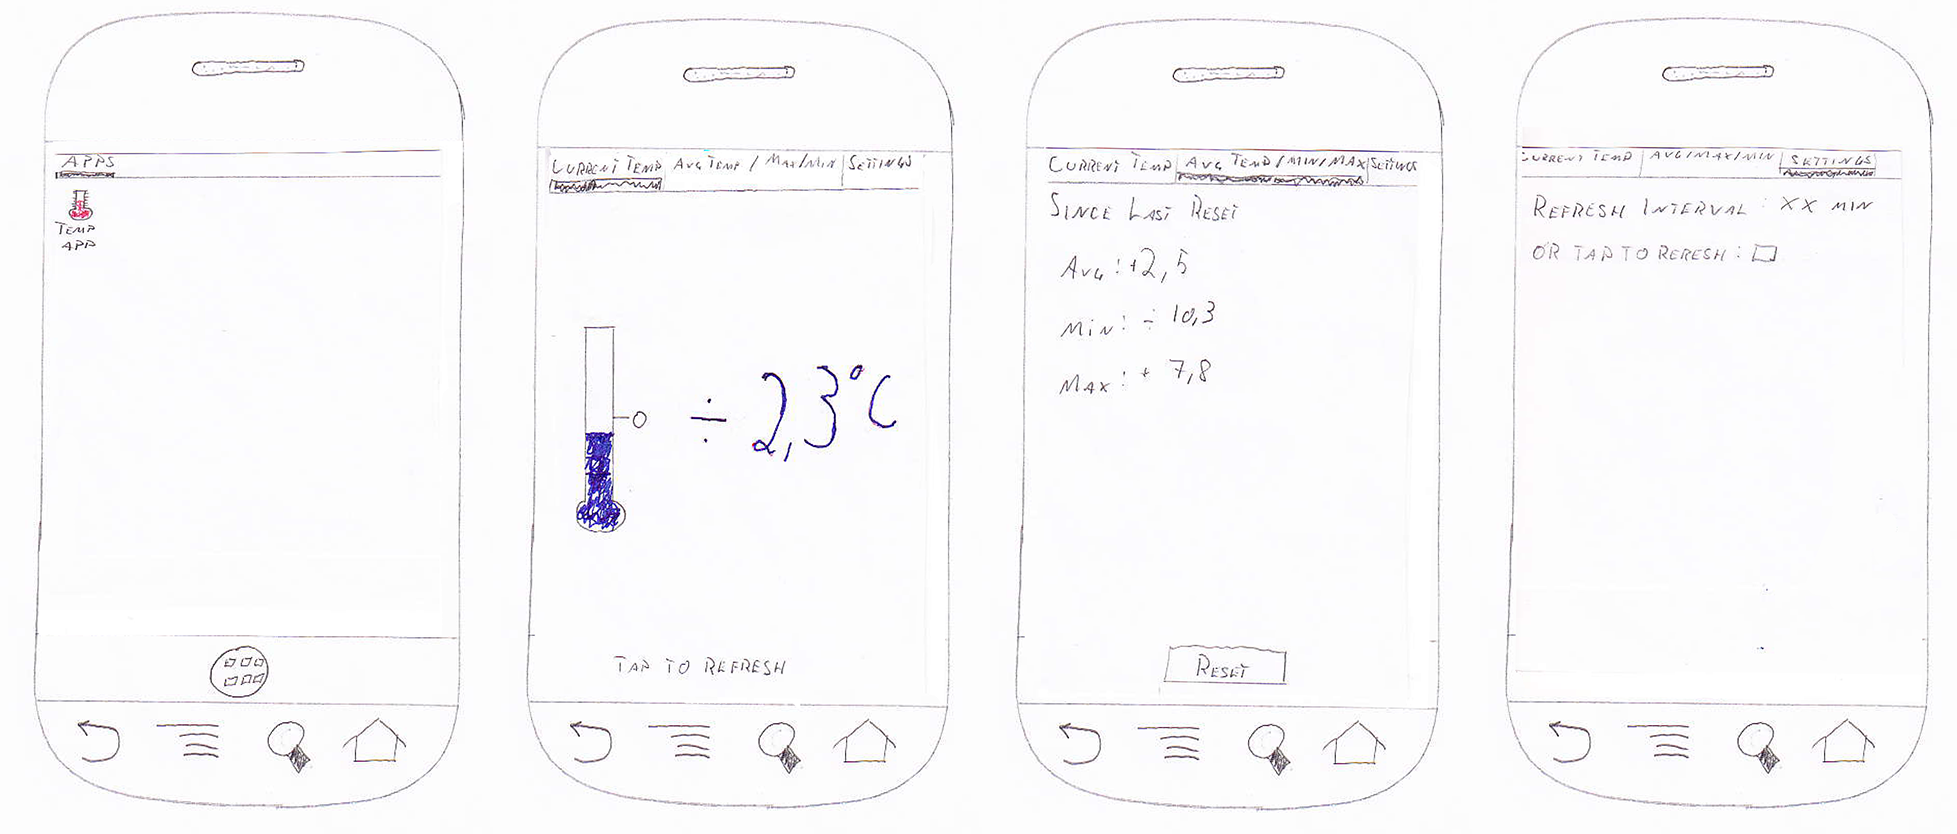
\includegraphics[width=1.0\textwidth]{img/prototype2-paper.png}
\caption{Paper Prototype for the temperature sensor.}
\label{fig:prototype2-paper}
\end{figure}

\begin{figure}[H]
\centering 
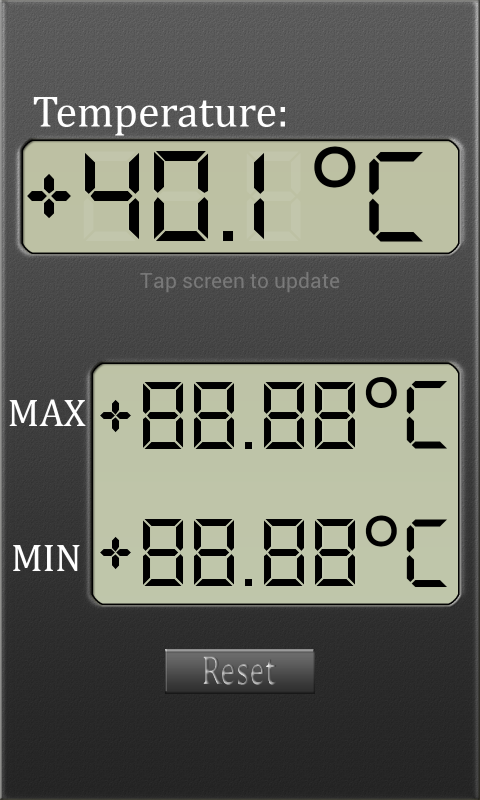
\includegraphics[width=0.3\textwidth]{img/prototype2-gui.png}
\caption{Final GUI design for the temperature prototype.}
\label{fig:prototype2-gui}
\end{figure}

\subsection{oSNAP BlingLED Application}
\begin{wrapfigure}{l}{20mm}
	\centering 
\includegraphics[scale=0.25]{img/app-led}
\end{wrapfigure}
This application uses ComLib to connect to the third prototype, the LED Matrix (see section \ref{section:prototype-led}).
It allows the user to control the color of each LED in the matrix wirelessly through Bluetooth.
This is yet another showcase for how the ComLib can be integrated into any application.
Figure \ref{fig:design-ledmatrix} shows the Android application used to control the prototype.

\begin{figure}[h!]
	\begin{center}
	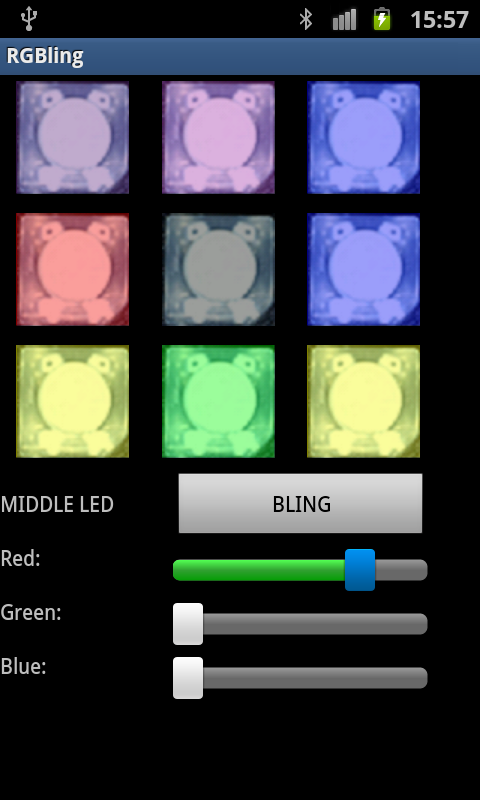
\includegraphics[scale=0.35]{img/prototype3rgBling.png}
	\end{center}
	\caption{Concept of the Android application BlingLED.}
	\label{fig:design-ledmatrix}
\end{figure}

\subsection{oSNAP Twitter application}
\begin{wrapfigure}{l}{20mm}
	\centering 
\includegraphics[scale=0.25]{img/app-twitter}
\end{wrapfigure}
Similar to the Facebook application (see section \ref{section:service-fb}),
except that it is a Twitter specific implementation that is able to read NTNU's public Twitter page.

\section{Prototypes}
\label{sec:prototypes}
Three different prototypes will be produced for the project. Their purpose is to show that the libraries can effectively simplify the prototyping of Arduino-based TUI.
One of the prototypes, the oSNAP Jacket (formerly the T-Shirt), is significantly bigger and more complex than the other two.
The oSNAP Jacket is the main prototype of the project; the purpose of the other two
is just to show that the libraries can be use for other applications and in different contexts - to showcase the generic nature of our libraries.

\subsection{Prototype 1: The oSNAP Jacket}
This is our main prototype and will showcase a lot features.
It consists of a Jacket connected to an Arduino Fio (figure \ref{fig:design-arduinofio}). The original prototype featured a different
Arduino micro-controller called the Arduino Lilypad (figure \ref{fig:design-arduinolilypad}). The Lilypad is optimized for sewing into 
clothing in both size and structure in addition to being washable. We discarded the Lilypad after we changed from T-Shirt to Jacket,
since in the Jacket we did not need to sew the components using conductive thread and washing was not a priority. In addition the 
Arduino Fio offered additional advantages such as connector for a battery pack, smaller size, better prototyping and a charger.

%the following magic allows images to be drawn side by side
\begin{figure}[H]
	\begin{minipage}[b]{0.5\linewidth}
		\centering
		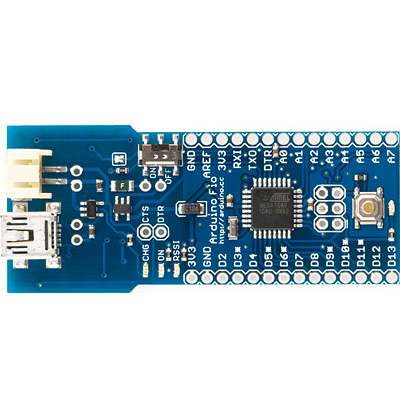
\includegraphics[scale=0.35]{img/design-arduinofio.png}
		\caption{The Arduino Fio \cite{link:arduino-fio}}
		\label{fig:design-arduinofio}
	\end{minipage}
		\hspace{0.5cm}
	\begin{minipage}[b]{0.5\linewidth}
		\centering
		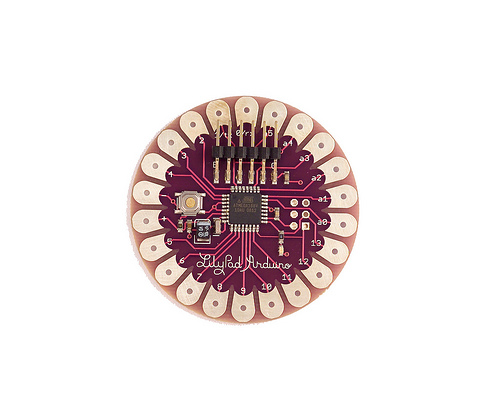
\includegraphics[scale=1.50]{img/design-arduinolilypad}
		\caption{The Arduino Lilypad \cite{link:arduino-lilypad}}
		\label{fig:design-arduinolilypad}
	\end{minipage}
\end{figure}

The application of this prototype will feature several displays and indicators which will receive social data through an Android phone.
The jacket features different tangible interfaces (see figure \ref{fig:design-TShirt}):
	
\begin{itemize}
	\item LEDs
	\item LCD Display
	\item Sound speaker
	\item Vibration module
\end{itemize}

\begin{figure}[H]
	\begin{center}
	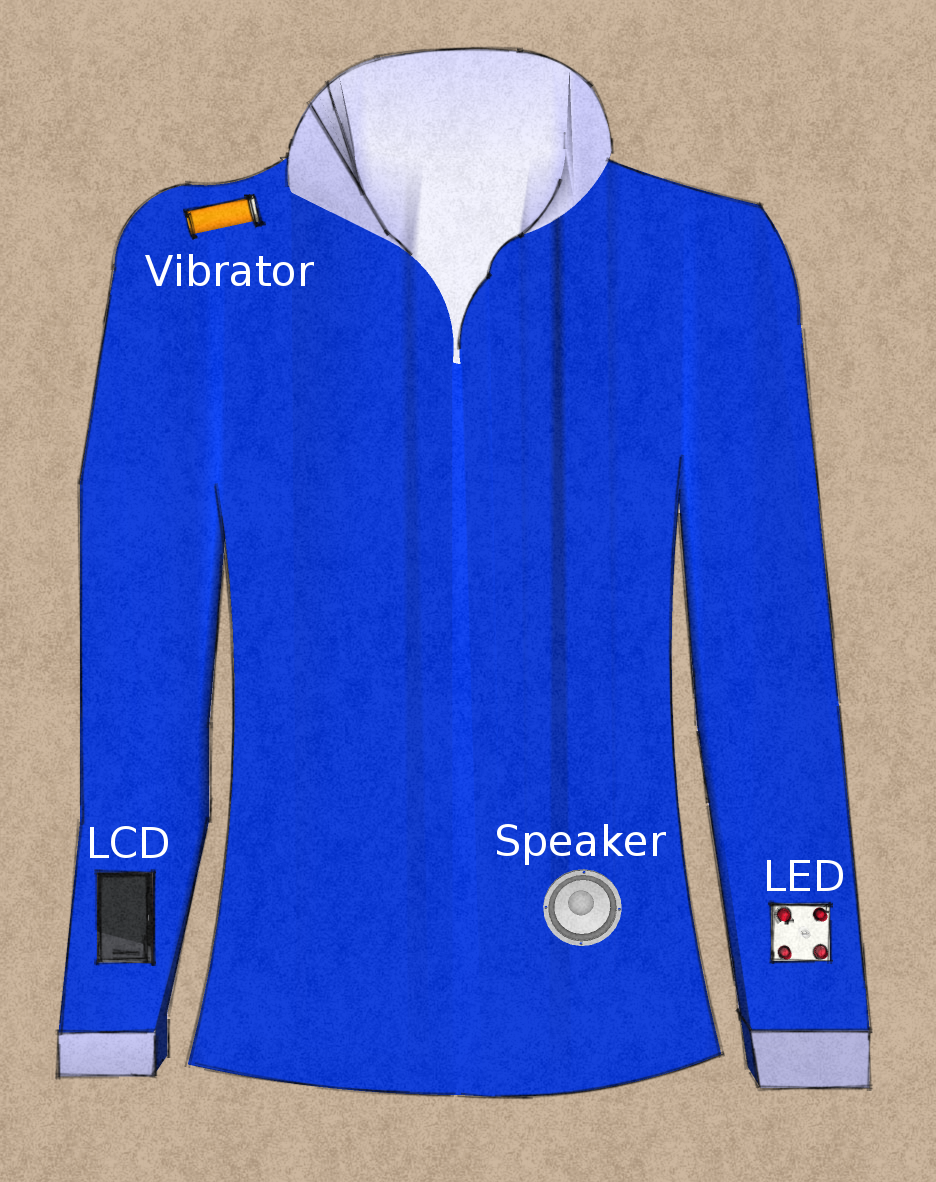
\includegraphics[scale=0.2]{img/design-tshirtproto}
	\end{center}
	\caption{Concept drawing of the Jacket Prototype}
	\label{fig:design-TShirt}
\end{figure}
	
Any of these can be mapped to a fair deal of concepts found in social networks.
So a "Poke" from Facebook could become a vibration on the Jacket. When someone "Likes" your post a small sound effect
could be played, a LED blinking on status updates from Twitter, etc. The Jacket is connected to the social networks
through wireless connection with an Android mobile. Specifically, the Android mobile is connected to the Internet
and carried in the pocket of the person using the Jacket. The jacket is connected wirelessly with the Arduino Fio through Bluetooth.

	
\subsection{Prototype 2: Temperature Sensor for Android} \label{section:prototype-temp}
This prototype will primarily showcase the communication from Arduino to Android using our libraries. 
Figure \ref{fig:design-temperature} shows a visual representation of the entire Temperature Sensor
prototype with an Android device connected wirelessly through bluetooth to the Arduino board. The 
Arduino unit can read the ambient temperature and be able to send this info to an Android application,
 either on demand or at a set interval that can be chosen through settings in the application. Figure \ref{fig:design-temperature-schematic} describes how the hardware in this prototype is connected and which parts are required to build it.

\begin{figure}[h!]
	\centering
	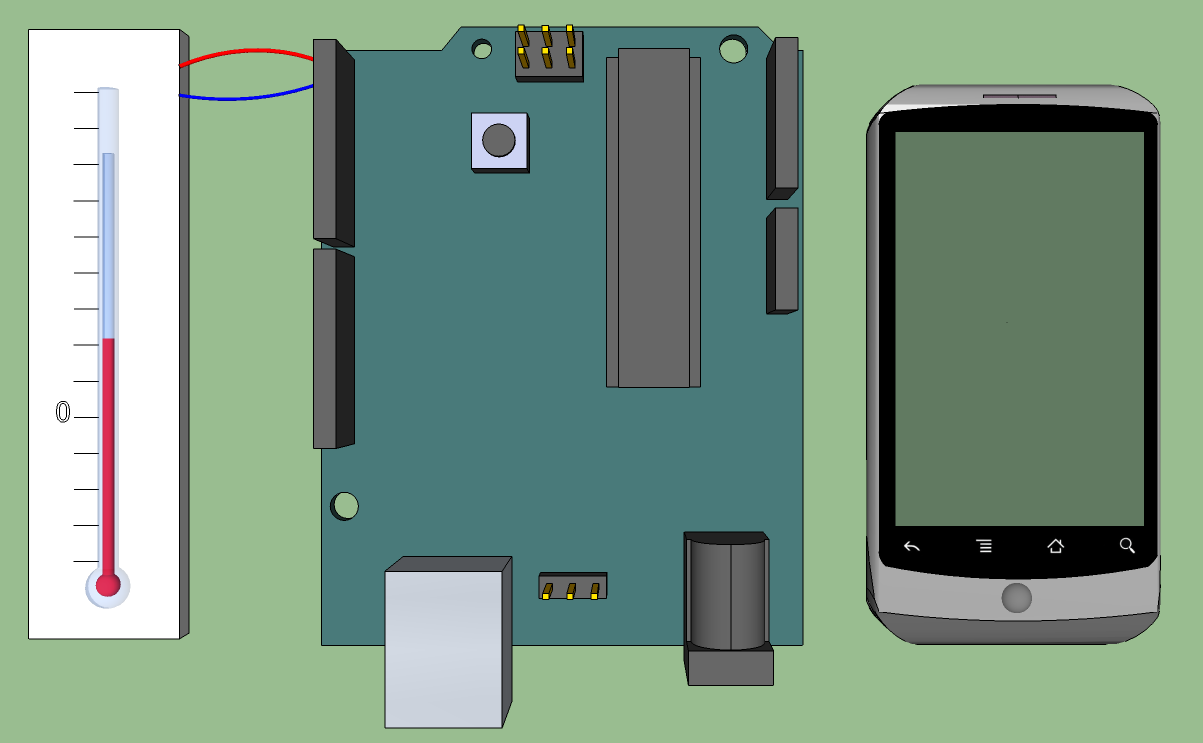
\includegraphics[scale=0.35]{img/design-temperature}
	\caption{Concept drawing of the temperature application setup.}
	\label{fig:design-temperature}
\end{figure}

\begin{figure}[h!]
	\centering
	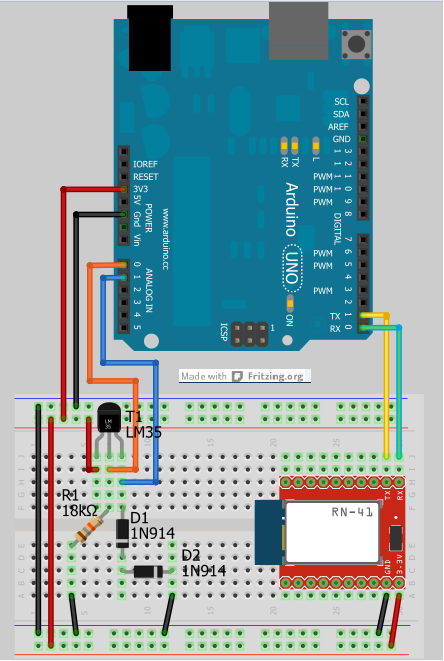
\includegraphics[scale=0.5]{img/tempapp-schematic}
	\caption{Schematic for hardware setup in the Temperature prototype}
	\label{fig:design-temperature-schematic}
\end{figure}
	
\subsection{Prototype 3: LED Matrix} \label{section:prototype-led}
This prototype was first planned to be LED lights showing what mood you had on MySpace.
Red LED lights would be angry, green would be happy and so on. We discovered that MySpace had removed this feature from their pages, even though it is still supported by the API. It would be a fools errand to pursue something you could not test properly
in a real world situation, so we changed the concept of this prototype. It ended up to be a prototype with LEDs governed by Android.
You select colors of the 3x3 LEDS in a graphical interface in an Android app. Then you send this information over Bluetooth
to the Arduino which displays the selected colors on a necklace.
The purpose of this prototype is to show how easy it is to implement the Communication Library in an Android application and how most of the time can be spent on actual development rather than understanding the specifics of the library. The second purpose is to show the extensibility of using Shift Registers to control a multitude of components. This prototype is using four shift registers to control nine LEDs but it could theoretically be several thousand with more shift registers and chained Arduino boards. An external open-source library was used to control the shift registers\cite{link:shiftpwm}.  Figure \ref{fig:design-blingled-schematic} describes how the hardware in this prototype is connected and which parts are required to build it.

\begin{figure}[h!]
	\centering
	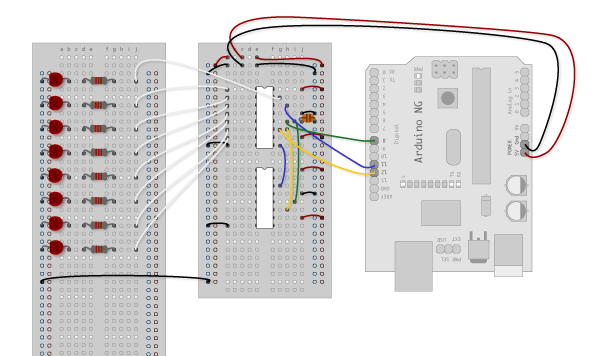
\includegraphics[scale=1.0]{img/blingled-schematic}
	\caption{Schematic for hardware setup in the BlingLED prototype}
	\label{fig:design-blingled-schematic}
\end{figure}


\section{Package Structure}
The source code of the whole system can be organized in smaller sections.
Here we describe some of the packages we have divided the system code into.
The system was coded in Arduino C and Java. Java was used to code Android libraries and applications.
Arduino C code is executed on the Arduino board. The Java code is again divided into packages.
Below is a brief description of the most important ones.

\subsection{Java code}
\begin{itemize}
	\item \textbf{no.ntnu.osnap.com}\newline
		The Communication Library contains every class to establish connection with a remote device using a generalized
		protocol interface. The actual details of the communication such as Bluetooth, cable, WiFi, stream-based or
		sockets are hidden away from the user. This is to provide a simple and generic interface to all supported
		communication methods. The user can easily add new communication types by extending an abstract class.
		The ComLib additionally defines a standard of storing and retrieving meta-data of services and download URL
		links from the remote device using JSON.
	\item \textbf{no.ntnu.osnap.com.testing}\newline
		Test units and sample programs for the ComLib. These are simple test applications that are run on
		the Android to test if the ComLib is working correctly using the specified
		protocol.
	\item \textbf{no.ntnu.osnap.social}\newline
		Social library main classes. These can send requests for data from social networks. The listener package (see below) 
		handles the responses from these requests.
	\item \textbf{no.ntnu.osnap.social.models}\newline
		Social library data models. These are common models representing data from social networks such as message, person,
		notification or group.
	\item \textbf{no.ntnu.osnap.social.listeners}\newline
		Social library listeners. Includes listeners for any response on requests for social networks.
	\item \textbf{no.ntnu.osnap.mockups}\newline\label{section:mockup}
		Sample and 'driver' applications used for testing purposes.
		Also includes example applications for third-party developers.
	\item \textbf{no.ntnu.osnap.tshirt, no.ntnu.osnap.temp, no.ntnu.osnap.pixelleds}\newline
		These packages contain Android applications (called Activities in the Android terminology) for the three prototypes
		we have implemented. Activity resources (graphics, sounds and activity manifest) are also included in these packages.
	\item \textbf{no.ntnu.osnap.facebook, no.ntnu.osnap.twitter}
		These packages contain the Facebook and Twitter social services.
\end{itemize}

\subsection{Arduino C code}
All the Arduino code is in one class called \emph{ComputerSerial}, and there is therefore no package structure to speak of.
The class consists of a header file and a source file. These two files can be included in any Arduino projects that want to use our protocol for communication.

\section{oSNAP Market}
As we approached the final sprint, it became apparent that we needed a way to simplify the end user experience. The oSNAP Market is a simple market made for the purpose of prototyping oSNAP compatible apps' distribution and interaction.  See \ref{section:app-generic} for an example of real life usage of the \emph{oSNAP Market}. It follows a simple MVC scheme, where each part can easily be changed.

The market does not currently rely on any server side scripting. For the purpose of internal testing, the market (see figure \ref{fig:market-screen}) is currently being hosted at \newline http://folk.ntnu.no/svarvaa/utils/pro2www.

\subsection{Model}
The model is a simple JSON object with some required data fields. The model, or back-end, can be swapped out with anything, as long as it supplies the view with a JSON object following the pattern in the source code excerpt below.
\javacode
\begin{lstlisting}
var market = {
    "apps": [{
        // Required
        "id": 0,
        // Required
        "title": "OSNAP(app)",
        // Optional
        "icon": "icon/osnap/icon128.png",
        // Optional
        "url": "apk/OsnapApp.apk",
        // Required
        "about": "Generic app for testing OSNAP-compatible arduino products.",
        // Optional
        "deps": [50]
    }, {
        "id": 1,
        "title": "JacketApp",
        "icon": "icon/jacket/icon128.png",
        "url": "apk/Tshirt.apk",
        "about": "This is our main prototypes and will showcase a lot features...",
        "deps": [0, 4, 5]
    },
        ...
    }]
};
\end{lstlisting}

\subsection{Controller}
The controller receives an app, and the model from the view. It will then generate HTML for that app, while figuring out it's dependencies.

\subsection{View}
The view loops through every app in the model and generates a view using the controller. The resulting view is then inserted into the appList element's html, which is just an empty UL html element.

\begin{figure}
	\begin{center}
	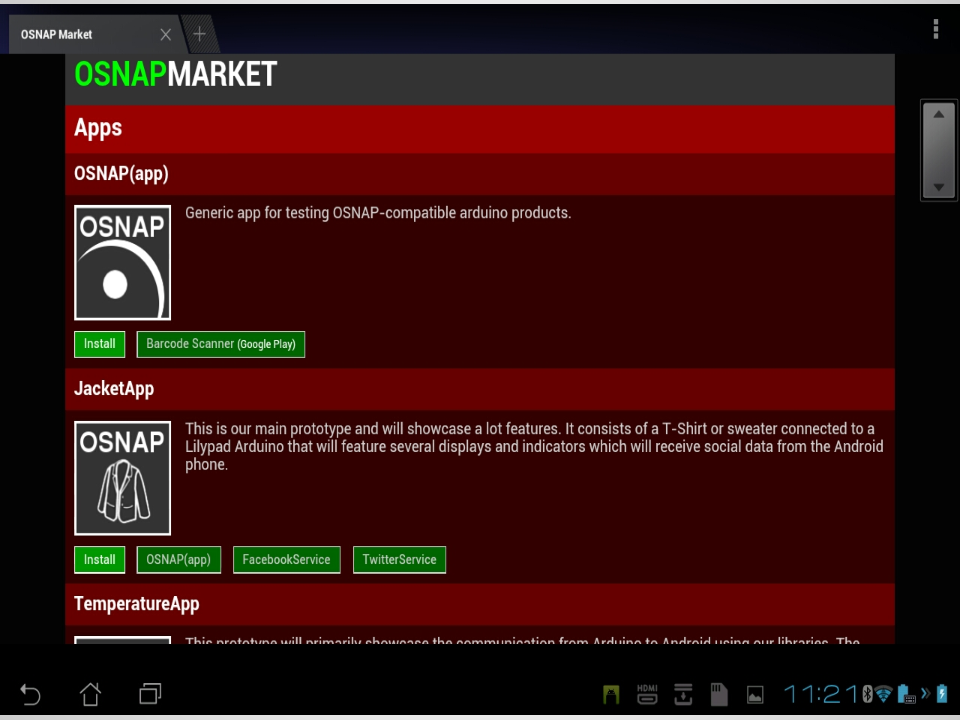
\includegraphics[scale=0.4]{img/market-screen.png}
	\end{center}
	\caption{Screenshot of the oSNAP Market running on an Android 4.0 device.}
	\label{fig:market-screen}
\end{figure}
